\documentclass[12pt]{article}
%\usepackage{amsmath}
\usepackage{mathtools}
\usepackage[a4paper, margin=1in]{geometry}
\usepackage{algpseudocode}
\usepackage{graphicx}
\graphicspath{ {./} }
%\usepackage{hyperref}
\usepackage[utf8]{inputenc}
\usepackage[english, russian]{babel}
\usepackage[T1, T2A]{fontenc}


%\title{Getting started}
%\author{Veloci Raptor}
%\date{03/14/15}

\begin{document}
%\maketitle

Робота викладеного методу для структури з параметрами $k=3$ та $m=3$ може бути проілюструвати на такому прикладі (рис. \ref{fig:ex1}).
Комірки з невизначеним станом $(-1)$ зображені як пусті комірки.

Нехай вектор $Y$ заданий і має значення $Y = \{ 2, 3, 5 \}$.

Отримання першого вектору $X_1$ виконується наступним чином.

Перед початком роботи всі комірки мають невизначений стан (пусті).

Згідно з пунктами 2 та 3 запропонованого методу, в якості поточного шару вибирається останній ($i = m - 1 = 2$), після чого для кожного ФП$_j$ в ньому знаходиться адреса $v_{2, j}$ пустої комірки. Нехай були вибрані комірки $v_{2,1}=2, v_{2,2}=1, v_{2,3}=2, v_{2,4}=3$.

Здійснюється перехід до попереднього шару: $i = i - 1 = 1$ (пункт 4).

У відповідності до пункту 5, так як у ФП$_1$ є тільки пусті комірки, то вибирається будь-яка з них.
Нехай вона має адресу $v_{1,1}=1$, і нехай її значення $w_{1,1}=7$.
До ФП$_1$ записується $f_1(1)=7$.

Згідно пункту 6, за формулою $w_{i,j} = w_{i,j-1} \oplus v_{i+1,j-1}$ послідовно визначається решта значень $w_{1,j}$ в першому шарі зліва направо, а саме: $w_{1,2} = 7 \oplus 2 = 5, w_{1,3} = 5 \oplus 1 = 4, w_{1,4} = 4 \oplus 2 = 6, w_{1,5} = 6 \oplus 3 = 5$.
При цьому, так як відповідні ФП$_j$ мають тільки пусті комірки, то значення $v_{1,j}$ для них вибираються випадковим чином, наприклад: $v_{1,2} = 2, v_{1,3} = 3, v_{1,4} = 1, v_{1,5} = 2$, а значення цих комірок визначаються відповідним знайденим $w_{1,j}$: $f_2(2)=5, f_3(3)=4, f_4(1)=6, f_5(2)=5$.

Так як поточний шар э першим ($i=1$), то прохід нагору завершується (згідно пункту 7).

Відповідно до 8-го пункту, компоненти вхідного вектора $X_1$ визначаються як значення на вході відповідних ФП в першому шарі: $x_{1,1}=v_{1,1}=1, x_{1,2}=v_{1,2}=2, x_{1,3}=v_{1,3}=3, x_{1,4}=v_{1,4}=1, x_{1,5}=v_{1,5}=2$.

Згідно пункту 9, для ФП$_1$ в останньому шарі довільним чином вибирається значення комірки, адреса якої $v_{2,1}=2$ була визначена раніше. Нехай це значення $w_{2,1}=4$. До ФП$_1$ записується $f_1(2)=4$.

За формулою $w_{m-1,j}=(x_{q,j-1} \oplus y_{j-1}) \oplus w_{m-1,j-1}$ послідовно знаходиться решта значень комірок в останньому шарі, відповідні адреси яких були визначені раніше: $w_{2,2} = (1 \oplus 2) \oplus 4 = 7, w_{2,3} = (2 \oplus 3) \oplus 4 = 5, w_{2,4} = (3 \oplus 5) \oplus 6 = 0$.

Таким чином, отримано значення вектора $X_1=\{1,2,3\}$ і завершено один повний прохід методу.

Так як в кожному ФП залишилося хоча б 2 комірки з невизначеним станом, то можна продовжувати формування наступних векторів $X$.

\begin{figure}[h]
\centering
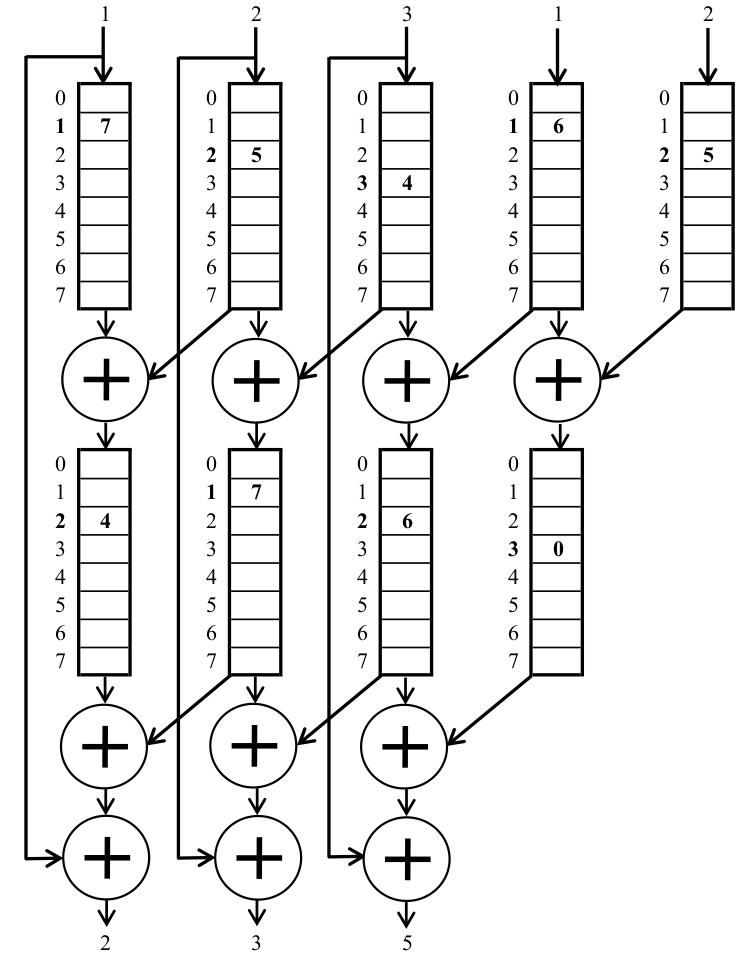
\includegraphics[width=0.6\textwidth]{ex1}
\caption{Результат одного проходу метода}
\label{fig:ex1}
\end{figure}

\newpage

В цій статті прийняті такі умовні позначення:
\begin{enumerate}
\item $n$ -- довжина вектора;
\item $k$ -- розрядність фрагмента;
\item $m = \frac{n}{k}$ -- кількість фрагментів;
%TODO
\item $X = \{x_1, x_2, \dotsc , x_m\}$ -- вхідний вектор, $\forall i=1,2 \ldots m : x_i \in \{0,1, \ldots ,2^k-1\}$;
\item $Y = \{y_1, y_2, \dotsc , y_m\}$ -- вихідний вектор, $\forall i=1,2 \ldots m : y_i \in \{0,1, \ldots ,2^k-1\}$;
\end{enumerate}

Будь-який функціональний перетворювач (ФП) можна представити у вигляді таблиці з $2^k$ рядків. Тоді значенням на вході до ФП буде називатися адреса комірки з цієї таблиці, а значенням на виході з ФП - числове значення цієї комірки.

В подальшому описі через $v_{i,j}$ позначено значення на вході j-го ФП на i-му шарі, а через $w_{i,j}$ - значення на виході: $f_j(v_{i,j}) = w_{i,j}$.

Вихідний вектор Y вважається заданим.

Пропонований метод передбачає наступну послідовність дій для формування векторів Х:

\begin{enumerate}
\item Всі комірки всіх ФП заповнюються значенням $-1$, що відповідає невизначеному стану: $\forall j=1,2 \ldots 2m-1, l=0,1 \ldots 2^k-1 : f_j(l) = -1$.
\item \label{itm:start} В якості поточного шару вибрати останній: $i=m-1$.
\item \label{itm:findundef}Для кожного ФП$_j$ в останньому шарі $(j=1,2 \ldots m+1)$ знаходиться адреса комірки $v_{m-1,j}$, для якої стан ФП$_j$ невизначений.
\item \label{itm:goprev} Перейти до попереднього шару: $i=i-1$.
\item В першому ФП$_1$ шукається адреса $v_{i,1}$ комірки, для якої стан ФП$_1$ визначений: $f_1(v_{i,1}) \neq -1$;
якщо такої комірки немає, то адреса $v_{i,1}$ і відповідне значення $w_{i,1}$ комірки вибираються довільним чином, а до ФП$_1$ записується $f_1(v_{i,1})=w_{i,1}$.
\item Для решти ФП$_j$ в поточному шарі $(j=2,3 \ldots 2m-i)$ послідовно визначаються значення на виході $w_{i,j}$ за такою формулою: $w_{i,j} = w_{i,j-1} \oplus v_{i+1,j-1}$;
при цьому адреса $v_{i,j}$ комірки ФП$_j$ вибирається випадковим чином серед тих, для яких значення комірки визначене і дорівнює знайденому $w_{i,j}$ $(f_j(v_{i,j})=w_{i,j})$;
якщо комірок зі значенням $w_{i,j}$ у ФП$_j$ немає, то береться будь-яка комірка $v_{i,j}$ з невизначеним станом і її значення визначається знайденим $w_{i,j}$: $f_j(v_{i,j})=w_{i,j}$.
\item Якщо номер поточного шару $i \geq 2$, тобто поточний шар не є першим, то здійснюється перехід на повторне виконання пункту \ref{itm:goprev}.
\item Значення компонентів $q$-го вхідного вектора $X_q$ визначаються як значення на вході відповідних ФП в першому шарі: $x_{q,j}=v_{1,j}$ $(j=1,2 \ldots 2m-1)$.
\item Для першого ФП$_1$ в останньому шарі довільним чином вибирається значення $w_{m-1,1}$ комірки, адреса $v_{m-1,1}$ якої була визначена в пункті \ref{itm:findundef}, і вибране значення записується в ФП$_1$ за відповідною адресою: $f_1(v_{m-1,1})=w_{m-1,1}$.
\item Для решти ФП$_j$ в останньому шарі $(j=2,3 \ldots m+1)$ послідовно знаходяться значення $w_{m-1,j}$ комірок за відповідними адресами $v_{m-1,j}$, що були знайдені в пункті \ref{itm:findundef}: $w_{m-1,j}=(x_{q,j-1} \oplus y_{j-1}) \oplus w_{m-1,j-1}$. Значення ФП$_j$ визначається наступним чином: $f_j(v_{m-1,j}) = w_{m-1,j}$.
\item Для всіх ФП$_j$ $(j=1,2 \ldots 2m-1)$ знаходиться кількість невизначених в них комірок $u_j$: $u_j= \ldots$.
\item Якщо кількість невизначених комірок $u_j$ для всіх ФП$_j$ $(j=1,2 \ldots 2m-1)$ не менше $m-1$: $\forall j \in \{1,2 \ldots 2m-1\}: u_j \geq m-1$, то перейти до формування наступного вхідного вектора $X_q$: $q=q+1$, перехід на пункт \ref{itm:start}.
\item Всі невизначені значення всіх ФП заповнити випадковими числами в діапазоні $0,1 \ldots 2^k-1$.
\end{enumerate}

\end{document}

input\slash output

Not like this ... but like this:\\
New York, Tokyo, Budapest, \ldots
$\oplus$

Author Name \hfill \today

% +++++++++++++++++++++++++++++++++++++++++++++++++++++++++++++++++++++++++++++
Всі комірки всіх ФП заповнюються значенням $-1$, що відповідає невизначеному стану: $\forall i=1,2 \ldots 2m-1, j=0,1 \ldots 2^k-1 : f_i(j) = -1$.

В якості поточного шару вибрати останній: $i=m-1$.

Для кожного ФП$_j$ в останньому шарі ($j=1,2 \ldots m+1$) знаходиться комірка $v_{m-1,j}$, для якої стан ФП$_j$ невизначений.

\begin{algorithmic}
\For{$i=m-2,m-3 \ldots 1$}
	\State Довільним чином вибрати $v_{i,1}$, так щоб $f_1(v_{i,1}) \neq -1 $;
	\State якщо такого $v_{i,1}$ немає, то вибрати його і $w_{i,1}$ довільним чином
	\State і покласти $f_1(v_{i,1}) = w_{i,1}$.
	\For{$j=2,3 \ldots 2m-i $}
		\State $w_{i,j} = w_{i,j-1} \oplus v_{i+1,j-1}$
		\If{$i=1$ та $j>m$}
			\State Покласти $v_{i,j} = v_{i,j-m}$; якщо при цьому
			\State $f_j(v_{i,j}) \neq -1$ та $f_j(v_{i,j}) \neq w_{i,j}$ $=>$ \textbf{conflict},
			\State інакше покласти $f_j(v_{i,j}) = w_{i,j}$.
		\Else
			\State $v_{i,j}$ вибрати так, щоб $f_j(v_{i,j}) = w_{i,j}$; якщо такого немає,
			\State то вибрати його випадковим чином, щоб $f_j(v_{i,j}) = -1$,
			\State і покласти $f_j(v_{i,j}) = w_{i,j}$; якщо такого немає $=>$ \textbf{conflict}
		\EndIf
	\EndFor
\EndFor

\For{$j=1,2 \ldots 2m-1$}
	\State $x_j = v_{1,j}$
\EndFor

\State Вибрати $w_{m-1,1}$ довільним чином і покласти $f_1(v_{m-1,1}) = w_{m-1,1}$.

\For{$j=2,3 \ldots m$}
	\State $w_{m-1,j} = (x_j \oplus y_j) \oplus w_{m-1,j-1}$.
\EndFor
\end{algorithmic}

\vspace{2em}

Як результат роботи одного такого проходу, маємо сформований новий вектор $X$ та додатково заповнені ФП системи.
% +++++++++++++++++++++++++++++++++++++++++++++++++++++++++++++++++++++++++++++
